%% bare_conf.tex
%% V1.4b
%% 2015/08/26
%% by Michael Shell
%% See:
%% http://www.michaelshell.org/
%% for current contact information.
%%
%% This is a skeleton file demonstrating the use of IEEEtran.cls
%% (requires IEEEtran.cls version 1.8b or later) with an IEEE
%% conference paper.
%%
%% Support sites:
%% http://www.michaelshell.org/tex/ieeetran/
%% http://www.ctan.org/pkg/ieeetran
%% and
%% http://www.ieee.org/

%%*************************************************************************
%% Legal Notice:
%% This code is offered as-is without any warranty either expressed or
%% implied; without even the implied warranty of MERCHANTABILITY or
%% FITNESS FOR A PARTICULAR PURPOSE! 
%% User assumes all risk.
%% In no event shall the IEEE or any contributor to this code be liable for
%% any damages or losses, including, but not limited to, incidental,
%% consequential, or any other damages, resulting from the use or misuse
%% of any information contained here.
%%
%% All comments are the opinions of their respective authors and are not
%% necessarily endorsed by the IEEE.
%%
%% This work is distributed under the LaTeX Project Public License (LPPL)
%% ( http://www.latex-project.org/ ) version 1.3, and may be freely used,
%% distributed and modified. A copy of the LPPL, version 1.3, is included
%% in the base LaTeX documentation of all distributions of LaTeX released
%% 2003/12/01 or later.
%% Retain all contribution notices and credits.
%% ** Modified files should be clearly indicated as such, including  **
%% ** renaming them and changing author support contact information. **
%%*************************************************************************


% *** Authors should verify (and, if needed, correct) their LaTeX system  ***
% *** with the testflow diagnostic prior to trusting their LaTeX platform ***
% *** with production work. The IEEE's font choices and paper sizes can   ***
% *** trigger bugs that do not appear when using other class files.       ***                          ***
% The testflow support page is at:
% http://www.michaelshell.org/tex/testflow/



\documentclass[conference]{IEEEtran}
% Some Computer Society conferences also require the compsoc mode option,
% but others use the standard conference format.
%
% If IEEEtran.cls has not been installed into the LaTeX system files,
% manually specify the path to it like:
% \documentclass[conference]{../sty/IEEEtran}
\usepackage{booktabs} 
\usepackage{amsmath} 
\usepackage{amsfonts}
% \usepackage{algorithmicx}
% \usepackage{algorithm}
% \usepackage{algpseudocode}
\usepackage{graphicx}
\usepackage{dblfloatfix}
\usepackage{tikz}
\usetikzlibrary{arrows.meta,positioning,fit,backgrounds}
\usepackage{float}
\usepackage{caption}
\usepackage{subcaption}
\usepackage[dvipsnames]{xcolor}
\usepackage{titlesec}
% Blue centred section titles
\definecolor{ieeblue}{RGB}{0, 84, 166}
\titleformat{\section}{\normalfont\large\bfseries\color{ieeblue}\centering}{\thesection.}{0.5em}{}
\titleformat{\subsection}{\normalfont\normalsize\bfseries\color{ieeblue!80}}{\thesubsection}{0.5em}{}

\usepackage{amssymb}      % For additional mathematical symbols
% \usepackage{algpseudocode}% For pseudocode in algorithms


% Some very useful LaTeX packages include:
% (uncomment the ones you want to load)


% *** MISC UTILITY PACKAGES ***
%
%\usepackage{ifpdf}
% Heiko Oberdiek's ifpdf.sty is very useful if you need conditional
% compilation based on whether the output is pdf or dvi.
% usage:
% \ifpdf
%   % pdf code
% \else
%   % dvi code
% \fi
% The latest version of ifpdf.sty can be obtained from:
% http://www.ctan.org/pkg/ifpdf
% Also, note that IEEEtran.cls V1.7 and later provides a builtin
% \ifCLASSINFOpdf conditional that works the same way.
% When switching from latex to pdflatex and vice-versa, the compiler may
% have to be run twice to clear warning/error messages.






% *** CITATION PACKAGES ***
%
%\usepackage{cite}
% cite.sty was written by Donald Arseneau
% V1.6 and later of IEEEtran pre-defines the format of the cite.sty package
% \cite{} output to follow that of the IEEE. Loading the cite package will
% result in citation numbers being automatically sorted and properly
% "compressed/ranged". e.g., [1], [9], [2], [7], [5], [6] without using
% cite.sty will become [1], [2], [5]--[7], [9] using cite.sty. cite.sty's
% \cite will automatically add leading space, if needed. Use cite.sty's
% noadjust option (cite.sty V3.8 and later) if you want to turn this off
% such as if a citation ever needs to be enclosed in parenthesis.
% cite.sty is already installed on most LaTeX systems. Be sure and use
% version 5.0 (2009-03-20) and later if using hyperref.sty.
% The latest version can be obtained at:
% http://www.ctan.org/pkg/cite
% The documentation is contained in the cite.sty file itself.






% *** GRAPHICS RELATED PACKAGES ***
%
\ifCLASSINFOpdf
  % \usepackage[pdftex]{graphicx}
  % declare the path(s) where your graphic files are
  % \graphicspath{{../pdf/}{../jpeg/}}
  % and their extensions so you won't have to specify these with
  % every instance of \includegraphics
  % \DeclareGraphicsExtensions{.pdf,.jpeg,.png}
\else
  % or other class option (dvipsone, dvipdf, if not using dvips). graphicx
  % will default to the driver specified in the system graphics.cfg if no
  % driver is specified.
  % \usepackage[dvips]{graphicx}
  % declare the path(s) where your graphic files are
  % \graphicspath{{../eps/}}
  % and their extensions so you won't have to specify these with
  % every instance of \includegraphics
  % \DeclareGraphicsExtensions{.eps}
\fi
% graphicx was written by David Carlisle and Sebastian Rahtz. It is


% correct bad hyphenation here
\hyphenation{op-tical net-works semi-conduc-tor}


\begin{document}
%
% paper title
% Titles are generally capitalized except for words such as a, an, and, as,
% at, but, by, for, in, nor, of, on, or, the, to and up, which are usually
% not capitalized unless they are the first or last word of the title.
% Linebreaks \\ can be used within to get better formatting as desired.
% Do not put math or special symbols in the title.
\title{TaViT: A Temporal Vision Transformer for Treatment-Aware Longitudinal Glioma Volume Trajectory Analysis}


% author names and affiliations
% use a multiple column layout for up to three different
% affiliations
\author{\IEEEauthorblockN{Mohamed Boufafa, Belkacem Chikhaoui, Belkacem Khaldi}
\IEEEauthorblockA{Applied Artificial Intelligence Institute\\
TELUQ University, Montreal, Canada \\
belkacem.chikhaoui@teluq.ca
}

}


% make the title area
\maketitle

% As a general rule, do not put math, special symbols or citations
% in the abstract
\begin{abstract}
Tracking how a brain tumor changes over time, and why this matters, is one of the most clinically urgent problems in neuro-oncology, yet most deep learning tools still treat each MRI scan in isolation. We present TaViT, a modular, treatment-aware pipeline that models a patient's full longitudinal MRI history by incorporating the therapies they received and the molecular profile of their tumor. Applied to the MU-Glioma cohort (203~patients, 596~scans), our system comprises: (1)~a fine-tuned nnU-Net backbone (30.8M~parameters) that segments whole tumor, tumor core, and enhancing tumor with a mean Dice of~0.877; and (2)~TaViT, a Treatment-Aware Temporal Vision Transformer (3.06M~parameters) conditioned on per-scan treatment tokens and 26 molecular biomarkers, which models tumor subregion volume trajectories across all observed timepoints, reaching $R^2 = 0.918/0.953/0.952$ for the three subregions. External zero-shot evaluation on BraTS-PTG (559~patients, 1,620~scans) confirms generalization across sites. Ablation studies show that treatment conditioning alone drives a~$+31.3\%$ improvement in trajectory estimation performance. As a complementary visualization component, a conditional DDPM interpolates between consecutive segmentation pairs to generate smooth per-patient tumor evolution videos.
\end{abstract}

\IEEEpeerreviewmaketitle

% ============================================================================
\section{Introduction}
% ============================================================================

Gliomas are the most common malignant primary brain tumors, accounting for roughly 80\% of cases~\cite{stupp2005glioblastoma, osborn2022who}. Glioblastoma, the most aggressive form, carries a median survival of under 15~months even with surgery, radiotherapy, and temozolomide chemotherapy~\cite{stupp2005glioblastoma}; recurrence is nearly inevitable. To track disease course, clinicians rely on serial MRI scans assessed through the RANO criteria~\cite{wen2010rano}, yet in practice this review remains largely manual and rarely incorporates the full treatment and molecular context documented in the patient record.

Over the past decade, deep learning has transformed brain tumor segmentation. Tools such as nnU-Net~\cite{isensee2021nnunet} and SwinUNETR~\cite{tang2022swinunetr} can now delineate tumor subregions with radiologist-level accuracy, but only on a single scan at a time. They tell us \emph{where} the tumor is, not \emph{how it has been changing}. Physics-based reaction-diffusion models attempt to fill this gap but require manual calibration and ignore the effect of treatment entirely~\cite{liu2023tadiff}. GAN-based approaches can predict pre-operative tumor shapes~\cite{liu2023tadiff}, but again without any treatment conditioning. The most closely related work, TaDiff~\cite{liu2023tadiff}, is a meaningful step forward: it conditions a diffusion model on past MRI sequences and treatment history to synthesize realistic future scan appearances. However, TaDiff was trained on just 18 patients and tested on 5, it does not report volumetric trajectory metrics, and it does not incorporate patient molecular biomarkers such as IDH or MGMT status.

In this paper we ask: given a patient's full longitudinal MRI history, their treatment record, and their molecular profile, can we \emph{continuously model how tumor subregion volumes have evolved} across all observed timepoints, and make those trajectories clinically interpretable? Our three contributions are:

\begin{enumerate}
    \item \textbf{TaViT (Treatment-Aware Volume Trajectory Transformer):} A bidirectional Vision Transformer (3.06M parameters) that sees a patient's entire scan sequence at once, conditioned on 8-dimensional per-scan treatment tokens and 26-dimensional molecular biomarkers (IDH1, MGMT, EGFR, and others), and models whole-tumor, tumor-core, and enhancing-tumor volumes at every observed timepoint simultaneously. It achieves $R^2 = 0.918/0.953/0.952$ across the three subregions.

    \item \textbf{An 18-test evaluation battery:} A rigorous, multi-category benchmark covering morphological, temporal, and clinical metrics applied identically to CNN, ViT, and TaViT, demonstrating that static per-scan models fundamentally fail to capture temporal dynamics while TaViT resolves these failures.

    \item \textbf{Large-scale, multi-site validation:} We train on MU-Glioma (203~patients, 596~scans, nearly $9\times$ the size of TaDiff's training set) and validate zero-shot on BraTS-PTG~\cite{deverdier2024bratsptg} (559~unseen patients, 1,620~scans with expert ground-truth segmentations).
\end{enumerate}

As a complementary visualization component, we additionally demonstrate a conditional DDPM that interpolates between consecutive nnU-Net segmentation pairs, generating smooth per-patient tumor evolution videos between observed scan timepoints.


% ============================================================================
\section{Related Work}
% ============================================================================

\textbf{Brain Tumor Segmentation.}
The story of deep learning for brain tumor segmentation is largely the story of U-Net and its successors. V-Net~\cite{milletari2016vnet} extended the architecture to 3D volumes with a Dice-based loss, establishing the template that most subsequent work follows. nnU-Net~\cite{isensee2021nnunet} took a different route: rather than proposing a new architecture, it showed that a carefully self-configured training pipeline could outperform hand-crafted task-specific models, achieving Dice scores of approximately 0.889/0.850/0.820 for WT/TC/ET on BraTS~2020. SwinUNETR~\cite{tang2022swinunetr} brought transformer-based encoders into this space, pairing a Swin Transformer~\cite{liu2021swin} with a convolutional decoder and using large-scale self-supervised pretraining to reach state-of-the-art 3D segmentation accuracy. The MONAI framework~\cite{cardoso2022monai} has made both architectures accessible to the medical imaging community. Despite this progress, every one of these models is a \emph{snapshot} tool: it has no memory, no concept of yesterday's scan, and no way to know whether the patient received chemotherapy since their last visit.

\textbf{Temporal Modeling in Neuro-Oncology.}
Predicting how a glioma will grow is a problem that predates deep learning. Classical reaction-diffusion equations model tumor invasion and proliferation mechanistically, but they require patient-specific calibration that is impractical in routine clinical workflows~\cite{liu2023tadiff}. Early deep learning approaches used GANs to predict pre-operative tumor masks~\cite{liu2023tadiff}, but these still ignored treatment entirely. A more fundamental shift came with probabilistic generative models that acknowledge the inherent uncertainty in tumor trajectories. The clearest expression of this direction is TaDiff~\cite{liu2023tadiff}, which conditions a DDPM on a sequence of past MRI scans and treatment-day pairs to synthesize realistic future scan appearances and corresponding tumor masks simultaneously. TaDiff is an important advance \textemdash{} it demonstrated that treatment history can meaningfully guide a generative model of tumor progression. Its limitations, however, are precisely what motivate the present work: it was trained on 18 patients and tested on 5, operates on 2D slices rather than full 3D volumes, does not report volumetric metrics, and does not incorporate the patient-level molecular context (IDH, MGMT, EGFR) that is routinely collected at diagnosis.

\textbf{Transformers for Sequence and Feature Conditioning.}
The Vision Transformer~\cite{dosovitskiy2021vit} established that patch-level self-attention~\cite{vaswani2017attention} can match or exceed CNNs on image understanding tasks. Swin Transformers~\cite{liu2021swin} refined this with shifted-window attention for computational efficiency. For modeling sequences of variable length, ALiBi~\cite{press2022alibi} provides an elegant positional bias that decays with inter-token distance, allowing the model to generalize to sequence lengths unseen during training. FiLM~\cite{perez2018film} offers a complementary mechanism: feature-wise affine conditioning that lets an auxiliary signal (such as treatment status) modulate intermediate representations at every layer \textemdash{} a lightweight but powerful form of conditioning that we exploit in our DDPM.

\textbf{Diffusion Models.}
Ho~et~al.~\cite{ho2020ddpm} showed that iterative denoising with a learned Gaussian model could generate high-fidelity images competitive with GANs. Nichol and Dhariwal~\cite{nichol2021improved} further improved the framework with learnable variance schedules and a cosine noise schedule that avoids early-step singularities. In medical imaging, diffusion models have been applied to data augmentation, anomaly detection, and image translation, with TaDiff~\cite{liu2023tadiff} being the first to target longitudinal glioma MRI generation specifically. We build on the DDPM framework for a different sub-task: generating temporally interpolated segmentation maps between known scan-pair endpoints, rather than extrapolating pixel-level future appearances.



% ============================================================================
\section{Methodology}
\label{sec:methodology}
% ============================================================================

The proposed framework operates as a unified two-stage pipeline. First, a fine-tuned nnU-Net backbone segments each multi-parametric MRI scan into three distinct tumor subregions, extracting a structured 2,825-dimensional embedding that captures both spatial morphological features and volumetric descriptors. Second, our Treatment-Aware Temporal Vision Transformer (TaViT) ingests the full chronological sequence of these scan embeddings. By contextualizing this sequence with time-varying treatment tokens and diagnostic molecular profiles, TaViT jointly models the volume trajectories of all three tumor subregions across all observed visits. Finally, as a complementary visualization aid, a conditional Denoising Diffusion Probabilistic Model (DDPM) interpolates between consecutive segmentations, generating anatomically plausible intermediate frames that render continuous tumor evolution videos. Fig.~\ref{fig:pipeline} illustrates the overall flow.

\begin{figure*}[!t]
\centering
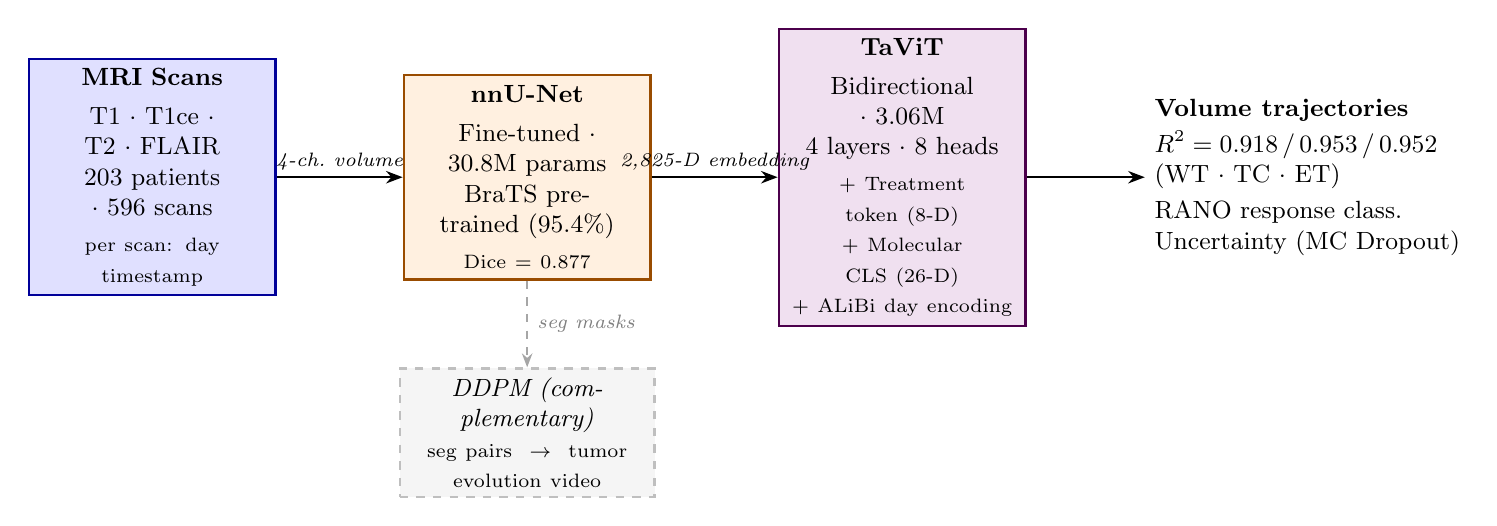
\begin{tikzpicture}[
  box/.style={rectangle, draw=#1!60!black, fill=#1!12, thick,
              minimum width=3.1cm, minimum height=2.6cm,
              align=center, text width=2.9cm, font=\small},
  arr/.style={-{Stealth[length=6pt]}, thick},
  darr/.style={-{Stealth[length=5pt]}, thick, dashed, gray!70},
  lbl/.style={font=\scriptsize\itshape, midway, above, inner sep=2pt},
  outbox/.style={align=left, font=\small}
]

%% ── Nodes ──────────────────────────────────────────────────────
\node[box=blue] (mri) {
  \textbf{MRI Scans}\\[3pt]
  T1 $\cdot$ T1ce $\cdot$ T2 $\cdot$ FLAIR\\
  203 patients $\cdot$ 596 scans\\[2pt]
  {\scriptsize per scan: day timestamp}
};

\node[box=orange, right=1.6cm of mri] (seg) {
  \textbf{nnU-Net}\\[3pt]
  Fine-tuned $\cdot$ 30.8M params\\
  BraTS pretrained (95.4\%)\\[2pt]
  {\scriptsize Dice = 0.877}
};

\node[box=violet, right=1.6cm of seg] (tav) {
  \textbf{TaViT}\\[3pt]
  Bidirectional $\cdot$ 3.06M\\
  4 layers $\cdot$ 8 heads\\[2pt]
  {\scriptsize + Treatment token (8-D)}\\
  {\scriptsize + Molecular CLS (26-D)}\\
  {\scriptsize + ALiBi day encoding}
};

\node[outbox, right=1.5cm of tav] (out) {
  \textbf{Volume trajectories}\\[2pt]
  $R^2 = 0.918\,/\,0.953\,/\,0.952$\\
  (WT $\cdot$ TC $\cdot$ ET)\\[2pt]
  RANO response class.\\
  Uncertainty (MC Dropout)
};

\node[rectangle, draw=gray!50, fill=gray!8, dashed, thick,
      minimum width=3.1cm, minimum height=1.1cm,
      align=center, text width=3.0cm, font=\small,
      below=1.1cm of seg] (ddpm) {
  \textit{DDPM (complementary)}\\
  {\scriptsize seg pairs $\;\to\;$ tumor evolution video}
};

%% ── Arrows ─────────────────────────────────────────────────────
\draw[arr] (mri)  -- node[lbl]{4-ch.\ volume} (seg);
\draw[arr] (seg)  -- node[lbl]{2,825-D embedding} (tav);
\draw[arr] (tav)  -- (out);
\draw[darr](seg.south) -- node[right, font=\scriptsize\itshape, gray]{seg masks} (ddpm.north);

\end{tikzpicture}
\caption{Overview of the proposed pipeline. A fine-tuned nnU-Net~\cite{isensee2021nnunet} segments each MRI scan and extracts structured 2,825-dimensional embeddings. TaViT processes the patient-level embedding sequence augmented with per-scan treatment tokens and a molecular marker CLS token, jointly modeling tumor subregion volumes at every observed timepoint. As a complementary component, a FiLM-conditioned DDPM~\cite{ho2020ddpm} interpolates between consecutive segmentation pairs to generate per-patient tumor evolution videos.}
\label{fig:pipeline}
\end{figure*}



\subsection{Segmentation and Embedding Extraction}

\subsubsection{nnU-Net Segmentation}
Building on the nnU-Net framework~\cite{isensee2021nnunet}, we fine-tune a PlainConvUNet (30.8M parameters) featuring a 6-stage encoder with channel widths [32, 64, 128, 256, 320, 320]. The model processes $128^3$ volumetric patches drawn from all four MRI contrasts and simultaneously predicts three binary segmentation masks (WT, TC, ET). Rather than training from random initialization, we load BraTS~2021~\cite{baid2021brats} pretrained weights, successfully transferring 209 of 219 available layers (95.4\% coverage), providing the model with a strong prior over glioma morphology before adapting it to our institutional longitudinal cohort.

Fine-tuning uses a soft Dice loss (sigmoid-activated, label smoothing $\delta = 10^{-5}$) optimized with AdamW~\cite{loshchilov2019adamw} ($\mathrm{lr} = 10^{-4}$, weight decay $10^{-5}$) under a cosine learning-rate schedule with a 5-epoch linear warmup. Training runs for 30 epochs on 429 scans, with 82 held out for validation, achieving a mean Dice of \textbf{0.877} (WT:~0.904, TC:~0.857, ET:~0.872).

To select the optimal backbone for downstream temporal modeling, we also fine-tuned SwinUNETR~\cite{tang2022swinunetr} under identical conditions. A systematic embedding quality evaluation (see \S\ref{sec:results}) consistently favored the CNN-derived representations across the majority of morphological and diversity metrics; accordingly, nnU-Net embeddings serve as input to TaViT in all experiments.

\subsubsection{Structured Embedding Extraction}
From each segmented scan, we extract a structured 2,825-dimensional embedding capturing complementary aspects of tumor morphology and spatial distribution. Neural encoder features (2,816-D) are derived by hooking the intermediate encoder stage (producing $16^3 \times 256$ feature maps), then applying two spatial pooling strategies within the tumor region of interest: \textbf{octant pooling} divides the ROI into a $2{\times}2{\times}2$ spatial grid and computes adaptive average pools in each of the 8 octants ($8 \times 256 = 2{,}048$-D), capturing coarse spatial heterogeneity; \textbf{mask-weighted regional pooling} computes weighted-mean features within each of the three tumor subregion masks ($3 \times 256 = 768$-D), encoding subregion-specific texture. Together these yield the 2,816-D neural representation.

These features are concatenated with a compact \textbf{9-dimensional morphological summary vector} comprising: three log-transformed subregion volumes $(\log(1{+}v)$ for WT, TC, ET), three binary presence flags (subregion volume $>10$ voxels), and three tumor burden ratios (TC/WT, ET/WT, ET/TC). This yields the final 2,825-D per-scan embedding.

Embeddings are extracted for all 571 successfully processed scans; complete-resection cases ($N=20$) retain zero-valued embeddings to preserve patient sequence integrity. Quantitative embedding quality analysis, including representational diversity and morphological encoding tests, is reported in \S\ref{sec:results}.


\subsection{Treatment-Aware Vision Transformer (TaViT)}

Rather than treating each scan in isolation, TaViT processes a patient's \emph{complete} longitudinal MRI history in a single forward pass, jointly estimating tumor subregion volumes across all observed timepoints while conditioning on the therapies received at each visit and the patient's molecular tumor profile.

\subsubsection{Architecture}
Each scan's neural embedding (2,816-D) is linearly projected to a shared 256-D token space. Three conditioning streams enrich each token:

\begin{itemize}
    \item \textbf{Treatment token} (8-D per scan): The active therapy combination is encoded as a binary vector, projected to 256-D, and added to the corresponding scan token, allowing the model to associate morphological changes with concurrent treatment.
    \item \textbf{Molecular CLS token} (26-D per patient): IDH, MGMT, EGFR, 1p/19q, ATRX, p53, and related markers are projected to 256-D via a dedicated MolProjector MLP and prepended as a shared classification token, providing stable per-patient biological context across all timepoints.
    \item \textbf{ALiBi temporal bias}~\cite{press2022alibi}: Real-valued calendar-day intervals are injected directly into the attention scores as head-specific negative linear biases:
    \begin{equation}
        \text{bias}(i, j) = -m \cdot \frac{|t_i - t_j|}{\tau}
    \end{equation}
    where $\tau = 180$~days normalises the temporal scale and $m$ is a head-specific slope, enabling the model to naturally attend more strongly to temporally proximate scans.
\end{itemize}

The enriched sequence passes through a 4-layer bidirectional Transformer encoder (8 heads, 256-D hidden, 512-D feedforward, dropout $p=0.2$), totalling \textbf{3.06M} parameters (backbone: 2.96M; MolProjector: 18K; volume decoder: 78K). A lightweight decoder projects each output token to three volumetric predictions (WT, TC, and ET volumes in millilitres) for every timepoint simultaneously.

\subsubsection{Training}
TaViT is trained with a four-component multi-task loss encoding three clinical priorities (volumetric accuracy, trajectory coherence, and response classification):
\begin{equation}
    \mathcal{L}_{\text{TaViT}} = \lambda_1 \mathcal{L}_{\text{vol}} + \lambda_2 \mathcal{L}_{\Delta} + \lambda_3 \mathcal{L}_{\text{cls}} + \lambda_4 \mathcal{L}_{\text{smooth}}
\end{equation}
$\mathcal{L}_{\text{vol}}$ is masked smooth-$\ell_1$ volume regression over all real timepoints; $\mathcal{L}_{\Delta}$ applies smooth-$\ell_1$ to consecutive volume changes for temporal coherence; $\mathcal{L}_{\text{cls}}$ is a class-weighted focal loss ($\gamma=2$) for RANO classification (patients with ${\geq}3$ timepoints); and $\mathcal{L}_{\text{smooth}}$ penalises biologically implausible volume oscillations. Weights: $\lambda_1=1.0$, $\lambda_2=0.5$, $\lambda_3=0.3$, $\lambda_4=0.05$.

Training uses AdamW~\cite{loshchilov2019adamw} ($\mathrm{lr}=10^{-3}$, weight decay $10^{-2}$, gradient clipping~1.0) with an 8-epoch warmup, across 3-fold stratified cross-validation (84 train / 43 val / 23 test patients; 120~epochs; patience~40). At inference, MC~Dropout~\cite{gal2016dropout} ($p=0.2$, $N=50$ passes) provides per-prediction uncertainty intervals.

\subsection{Conditional DDPM for Tumor Visualization}

As a complementary visualization aid, we train a conditional Denoising Diffusion Probabilistic Model~\cite{ho2020ddpm} to synthesize anatomically plausible intermediate segmentation frames between consecutive scan pairs, rendering each patient's tumor evolution as a smooth video.

The generator is a FiLM-conditioned~\cite{perez2018film} U-Net (DDPMv2, 24.7M parameters, $128{\times}128$ resolution) with base channel width $B=96$ and a cosine noise schedule ($T=50$ steps). Source and target segmentation masks condition the network via a CondEncoder that injects multi-scale scale-and-shift parameters into each decoder stage. Training uses 1,470 scan-pair triplets from 152 patients (1,250 train / 220 validation), with ET-rich triplets oversampled at $3{\times}$ to compensate for class imbalance, and runs for up to 300 epochs with early stopping (patience 35); the best checkpoint achieves a mean interpolation Dice of \textbf{0.760}. At inference, generated frames are post-processed to enforce the BraTS anatomical hierarchy ($\text{ET}\subseteq\text{TC}\subseteq\text{WT}$). For each patient, 15 interpolated frames per consecutive scan gap are overlaid on the T1ce MRI and rendered as MP4 videos at 3~FPS.


% ============================================================================
\section{Experiments}
\label{sec:experiments}
% ============================================================================
\subsection{Datasets}

\subsubsection{MU-Glioma (Primary Cohort)}
The primary dataset, MU-Glioma, is a curated longitudinal clinical cohort consisting of 203 glioma patients (596 total multi-parametric MRI scans including T1, T1ce, T2, and FLAIR) acquired at a single academic medical center. Each scan is paired with expert, hand-drawn segmentations outlining the three standard BraTS tumor subregions: whole tumor (WT), tumor core (TC), and enhancing tumor (ET). Consistent with real-world clinical distributions, the cohort is predominantly composed of WHO grade 4 glioblastoma (157 patients, 77.3\%), with astrocytoma (28, 13.8\%), diffuse glioma (10, 4.9\%), oligodendroglioma (4, 2.0\%), and pilocytic astrocytoma (3, 1.5\%) comprising the remaining cases.

To capture true temporal intervals, each scan is indexed by its calendar day relative to initial diagnosis. Among the 203 patients, 155 are tracked across multiple visits, with an average of 2.9 scans per patient (ranging from 1 to 6 timepoints). Each scan is annotated with an 8-dimensional binary treatment token encoding active therapies at that visit: temozolomide, radiotherapy, bevacizumab, lomustine, PCV, clinical trial enrollment, surgery, and corticosteroids. Each patient's baseline biology is represented by a 26-dimensional molecular marker vector collected at diagnosis, covering IDH1/IDH2 mutation status, MGMT promoter methylation, EGFR amplification, 1p/19q co-deletion, ATRX loss, p53 mutation, and related markers. Clinical response is defined using RANO-inspired criteria assigned per scan pair: progressive disease (46\%), partial response (25\%), stable disease (19\%), with 8\% single-scan cases and 2\% insufficient data.

\subsubsection{BraTS-PTG (External Validation)}
To evaluate the pipeline's robustness under realistic, multi-institutional clinical variance, we validate on the multi-site BraTS 2024 Post-Treatment Glioma (BraTS-PTG) dataset~\cite{deverdier2024bratsptg}, comprising 559 patients (1,620 total scans) with a significantly broader diagnostic spread, spanning glioblastoma (56.3\%), astrocytoma (17.4\%), oligodendroglioma (14.4\%), glioma NOS (10.1\%), and other subtypes (1.8\%). To counter calibration drift across scanner domains and clinical centers, we reserve 10 patients as a few-shot calibration cohort to optimize scale alignment; the remaining 549 patients serve as a fully held-out out-of-distribution test set.


\subsection{Implementation}
\label{sec:implementation}

All models were implemented in PyTorch and trained on NVIDIA Tesla T4 GPUs. The nnU-Net segmentation backbone was trained for 30 epochs using AdamW ($\mathrm{lr}=10^{-4}$, weight decay $10^{-5}$) with a cosine decay schedule. TaViT was trained for 120 epochs using AdamW ($\mathrm{lr}=10^{-3}$, weight decay $10^{-2}$, gradient clipping 1.0) under a 3-fold stratified cross-validation split (84 train / 43 validation / 23 test patients). The conditional DDPM was optimized for up to 300 epochs (early stopping patience 35) with a cosine noise schedule ($T=50$).

\subsubsection{Evaluation Protocol}
\label{sec:eval_protocol}

To rigorously assess both spatial embedding quality and longitudinal trajectory modeling, we use an \textbf{18-test validation battery} spanning four distinct clinical and representational categories:
\begin{itemize}
    \item \textbf{Morphological fidelity (M1--M6):} Evaluates how well the extracted embeddings preserve physical tumor characteristics. This includes volume correlation (M1), log-volume regression (M2), enhancing tumor fraction (M3), necrosis presence classification (M4), tumor core fraction (M5), and patient-level morphologic purity (M6).
    \item \textbf{Representational diversity (H1--H5):} Quantifies embedding coverage and information preservation. This includes effective rank via RankMe~\cite{garrido2023rankme} (H1), pairwise representation diversity (H2), first-scan clinical responder prediction (H3), and norm coefficient of variation (H4).
    \item \textbf{Temporal consistency (T1--T8):} Assesses the tracking of longitudinal dynamics. This includes whole-tumor volume drift (T1), visit temporal ordering correctness (T2), trajectory direction AUC (T3), baseline longitudinal RANO classification (T4), and trajectory monotonicity via Kendall's $\tau$ (T8).
    \item \textbf{Clinical utility (C1--C3):} Evaluates downstream prediction performance. This includes absolute subregion volume forecasting (C1), volume change direction (delta-sign) accuracy (C2), and RANO-defined clinical progression response classification (C3).
\end{itemize}

This battery is applied identically across CNN, ViT, and TaViT embeddings, enabling controlled comparison across architectures.




\subsection{Results}
\label{sec:results}

\subsubsection{Segmentation Performance}
Table~\ref{tab:segmentation} compares nnU-Net and SwinUNETR on MU-Glioma.

\begin{table}[h]
\centering
\caption{Segmentation Dice scores on MU-Glioma validation set.}
\label{tab:segmentation}
\begin{tabular}{lcccl}
\toprule
\textbf{Model} & \textbf{WT} & \textbf{TC} & \textbf{ET} & \textbf{Mean} \\
\midrule
nnU-Net (CNN)     & \textbf{0.904} & \textbf{0.857} & \textbf{0.872} & \textbf{0.877} \\
SwinUNETR (ViT)   & 0.855 & 0.827 & 0.848 & 0.843 \\
\bottomrule
\end{tabular}
\end{table}


\subsubsection{Temporal Test Battery}
We designed an 18-test evaluation battery covering morphological, temporal, and clinical metrics. Table~\ref{tab:temporal} shows the critical temporal tests where TaViT resolves CNN and ViT failures.

\begin{table}[h]
\centering
\caption{Temporal test results: CNN vs.\ ViT vs.\ TaViT.}
\label{tab:temporal}
\begin{tabular}{lccc}
\toprule
\textbf{Test} & \textbf{CNN} & \textbf{ViT} & \textbf{TaViT} \\
\midrule
T1: Volume drift $\rho$     & 0.023 & 0.028 & \textbf{0.608} \\
T4: RANO AUC                & 0.612 & 0.599 & \textbf{0.819} \\
T8: Kendall $\tau$           & 0.380 & 0.070 & \textbf{0.439} \\
\midrule
Tests passed (of 18)         & 11    & 8     & \textbf{14+3} \\
\bottomrule
\end{tabular}
\end{table}


\subsubsection{TaViT Volume Prediction}
Table~\ref{tab:tavit} presents TaViT's 3-fold cross-validated volume prediction performance.

\begin{table}[h]
\centering
\caption{TaViT volume prediction (3-fold CV on MU-Glioma).}
\label{tab:tavit}
\begin{tabular}{lcccc}
\toprule
& \textbf{WT} & \textbf{TC} & \textbf{ET} \\
\midrule
$R^2$        & \textbf{0.918} & \textbf{0.953} & \textbf{0.952} \\
MAE (mL)     & 15.52 & 4.67  & 3.69 \\
\bottomrule
\end{tabular}
\end{table}

The $\Delta$-sign accuracy (correctly predicting whether volume increases or decreases) reaches \textbf{83.3\%}. MC~Dropout uncertainty coverage is \textbf{83\%} ($N=50$).

\subsubsection{Ablation Study}
To quantify the impact of treatment history on trajectory estimation, we performed an ablation study by training an identical TaViT model without the 8-dimensional treatment conditioning token. The full model achieved a validation volume loss of 0.0640, compared to 0.0931 for the ablated baseline. This demonstrates that treatment conditioning alone drives a $+31.3\%$ improvement in trajectory estimation performance, confirming that the model actively leverages treatment context to refine its predictions rather than relying solely on imaging features.


\subsubsection{DDPM Video Generation}
The conditional DDPM achieves training Dice of 0.961/0.720/0.598 (WT/TC/ET, average~0.760). On the external BraTS-PTG dataset (1,032 unseen triplets from 109 patients), DDPM outperforms linear interpolation on all three subregions (average Dice 0.520 vs.\ 0.501, $+$1.9\%).


% ============================================================================
\section{Discussion}
\label{sec:discussion}
% ============================================================================

\textbf{CNN vs.\ ViT for single-scan morphology.}
Our results show that the CNN backbone (nnU-Net) captures superior per-scan morphological features compared to SwinUNETR, passing 11/14 cross-sectional tests versus 8/14. This is consistent with findings that self-configuring CNNs remain competitive with transformer-based architectures on domain-specific medical tasks~\cite{isensee2021nnunet}. Crucially, neither architecture alone can model temporal dynamics, motivating the TaViT layer built upon CNN embeddings.

\textbf{Treatment and molecular conditioning.}
TaViT's multi-modal conditioning is a key differentiator from prior work. While TaDiff~\cite{liu2023tadiff} incorporates treatment history into a diffusion model, our approach explicitly integrates 26-dimensional molecular markers (IDH1, MGMT, EGFR, etc.) via a dedicated MolProjector, providing richer patient context. The modular pipeline architecture also enables independent assessment: segmentation quality can be evaluated separately from temporal reasoning, and volume anchor features serve as clinically motivated structural priors analogous to measurements available during real follow-up workflows.

\textbf{Volume anchor transparency.}
TaViT receives segmentation-derived volumetric descriptors as part of its input, which are correlated with prediction targets. We frame this as a clinically integrated pipeline, analogous to radiomics workflows where segmentation measurements inform downstream prognostic models, rather than a pure latent predictor. This design choice is intentional and mirrors real clinical workflows where prior volumetric measurements are available during longitudinal assessment.

\textbf{Limitations.}
Our study has several limitations: (1)~MU-Glioma is a single-institution retrospective cohort of 203 patients; multi-center prospective validation is needed. (2)~The DDPM currently operates on 2D slices rather than full 3D volumes. (3)~TaViT-to-DDPM conditioning (using predicted future volumes to guide video generation) remains future work. (4)~Clinician qualitative assessment of generated videos has not yet been performed.


% ============================================================================
\section{Conclusion}
\label{sec:conclusion}
% ============================================================================

We presented a modular pipeline for treatment-aware longitudinal glioma modeling comprising CNN segmentation (nnU-Net, Dice~0.877), a temporal Vision Transformer (TaViT, $R^2 > 0.9$ for all subregions), and conditional DDPM video generation. TaViT resolves critical temporal test failures of static models by incorporating treatment tokens, molecular markers, and calendar-day ALiBi encoding. External validation on BraTS-PTG confirms generalization. Future work includes TaViT-conditioned video generation, prospective clinical validation, and clinician assessment of generated progression videos.


\bibliographystyle{IEEEtran}
\bibliography{ref}
\end{document}
